% Diagrama conceptual del enfoque híbrido (capítulo 1, §1.2).
% Dos vías a partir de la secuencia diaria: una baseline (cadena de Markov
% visible) y un predictor híbrido (HMM que alimenta a los modelos de ML), que
% se comparan en el análisis del error. Ilustrativo (no es figura de decisión).
% Compila standalone a PDF y se incluye con
% 
\includegraphics{figuras/intro_enfoque_hibrido.pdf}.
\documentclass[border=8pt]{standalone}
\usepackage[T1]{fontenc}
\usepackage[utf8]{inputenc}
\usepackage{lmodern}
\usepackage{tikz}
\usepackage{xcolor}
\usetikzlibrary{arrows.meta, positioning, calc, fit, backgrounds}

\definecolor{azul}{HTML}{1F4E79}
\definecolor{azulclaro}{HTML}{DAE8F5}
\definecolor{gris}{HTML}{555555}
\definecolor{grisclaro}{HTML}{ECECEC}
\definecolor{verde}{HTML}{2E7D32}
\definecolor{verdeclaro}{HTML}{E4F0E4}

\begin{document}
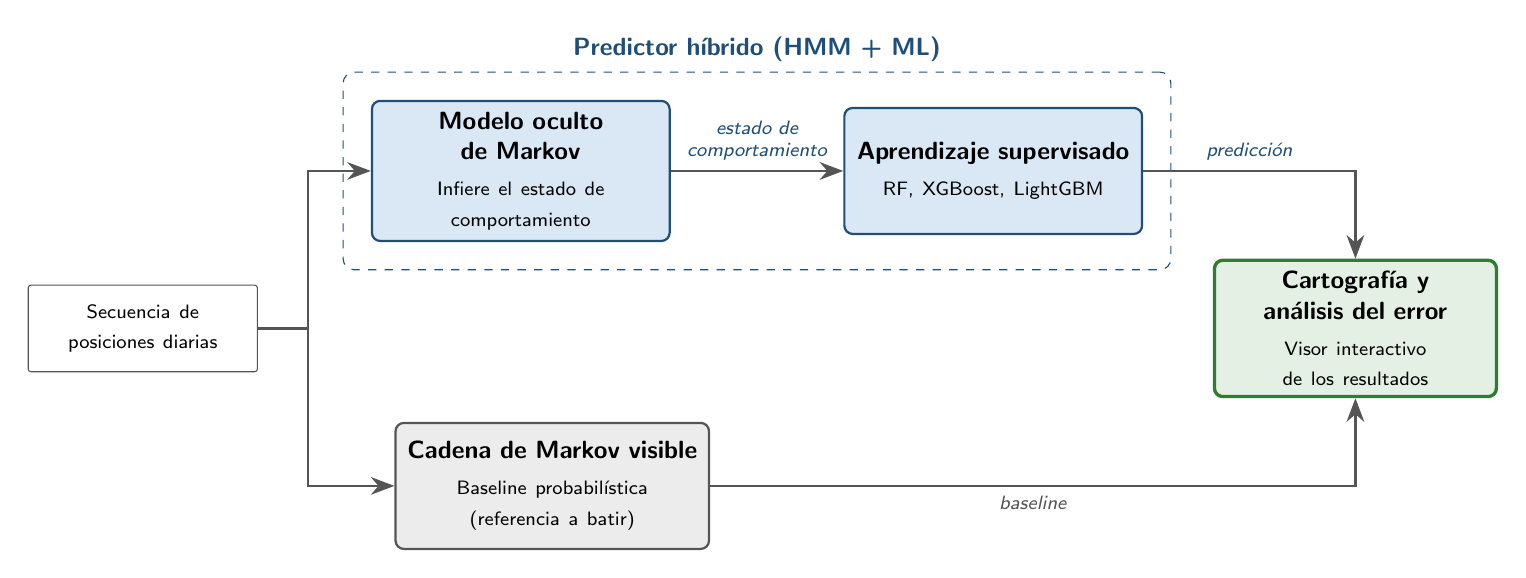
\begin{tikzpicture}[
  font=\sffamily\small,
  modelo/.style={rectangle, rounded corners=3pt, draw=azul, thick, fill=azulclaro,
                 text width=3.5cm, align=center, minimum height=1.6cm, inner sep=4pt},
  base/.style={rectangle, rounded corners=3pt, draw=gris, thick, fill=grisclaro,
                 text width=3.7cm, align=center, minimum height=1.6cm, inner sep=4pt},
  analisis/.style={rectangle, rounded corners=3pt, draw=verde, very thick, fill=verdeclaro,
                 text width=3.3cm, align=center, minimum height=1.6cm, inner sep=4pt},
  entrada/.style={rectangle, rounded corners=1pt, draw=gris, fill=white,
                 text width=2.7cm, align=center, minimum height=1.1cm, inner sep=3pt},
  arr/.style={-{Stealth[length=3mm]}, thick, gris},
  lin/.style={thick, gris},
  addlbl/.style={font=\sffamily\scriptsize\itshape, text=azul, align=center},
  baselbl/.style={font=\sffamily\scriptsize\itshape, text=gris, align=center},
]

% --- Entrada ---
\node[entrada] (in) at (0,0) {\scriptsize Secuencia de\\posiciones diarias};
\coordinate (b) at (2.1,0);

% --- Vía híbrida (arriba): HMM alimenta a los modelos de ML ---
\node[modelo] (hmm) at (4.8,2.0)  {\textbf{Modelo oculto de Markov}\\[2pt]\scriptsize Infiere el estado de comportamiento};
\node[modelo] (ml)  at (10.8,2.0) {\textbf{Aprendizaje supervisado}\\[2pt]\scriptsize RF, XGBoost, LightGBM};

% --- Vía baseline (abajo): cadena de Markov visible ---
\node[base] (mk) at (5.2,-2.0) {\textbf{Cadena de Markov visible}\\[2pt]\scriptsize Baseline probabilística (referencia a batir)};

% --- Análisis ---
\node[analisis] (viz) at (15.4,0) {\textbf{Cartografía y análisis del error}\\[2pt]\scriptsize Visor interactivo de los resultados};

% --- Ramas desde la entrada ---
\draw[lin] (in.east) -- (b);
\draw[arr] (b) |- (hmm.west);
\draw[arr] (b) |- (mk.west);

% --- Enlace interno de la vía híbrida ---
\draw[arr] (hmm) -- node[addlbl, above]{estado de\\comportamiento} (ml);

% --- Convergencia en el análisis ---
\draw[arr] (ml.east) -| node[addlbl, pos=0.25, above]{predicción} (viz.north);
\draw[arr] (mk.east) -| node[baselbl, pos=0.25, below]{baseline} (viz.south);

% --- Caja del predictor híbrido ---
\begin{scope}[on background layer]
  \node[draw=azul, dashed, rounded corners=4pt, inner sep=10pt, fit=(hmm)(ml),
        label={[azul, font=\sffamily\small\bfseries]above:Predictor híbrido (HMM + ML)}] {};
\end{scope}

\end{tikzpicture}
\end{document}
